%%%%%%%%%%%%%%%%%%%%%%%%%%%%
%                          %
% Luther Michaels          % 
% ECE 351-52               %
% Lab 4                    %
% September 30, 2021       %
% System Step Response     %
%    Using Convolution     %
%           Lab Report     %
%                          %
%%%%%%%%%%%%%%%%%%%%%%%%%%%%

%%%%%%%%%%%%%%%%%%%%%%%%%%%%%%%%%%%%%%%%%%%
%%% DOCUMENT PREAMBLE %%%
\documentclass[12pt]{report}
\usepackage[english]{babel}
\usepackage{url}
\usepackage[utf8x]{inputenc}
\usepackage{amsmath}
\usepackage{graphicx}
\graphicspath{{images/}}
\usepackage{parskip}
\usepackage{fancyhdr}
\usepackage{vmargin}
\usepackage{listings}
\usepackage{hyperref}
\usepackage{xcolor}

\definecolor{codegreen}{rgb}{0,0.6,0}
\definecolor{codegray}{rgb}{0.5,0.5,0.5}
\definecolor{codeblue}{rgb}{0,0,0.95}
\definecolor{backcolour}{rgb}{0.95,0.95,0.92}

\lstdefinestyle{mystyle}{
	backgroundcolor=\color{backcolour},   
	commentstyle=\color{codegreen},
	keywordstyle=\color{codeblue},
	numberstyle=\tiny\color{codegray},
	stringstyle=\color{codegreen},
	basicstyle=\ttfamily\footnotesize,
	breakatwhitespace=false,         
	breaklines=true,                 
	captionpos=b,                    
	keepspaces=true,                 
	numbers=left,                    
	numbersep=5pt,                  
	showspaces=false,                
	showstringspaces=false,
	showtabs=false,                  
	tabsize=2
}

\lstset{style=mystyle}

\setmarginsrb{3 cm}{2.5 cm}{3 cm}{2.5 cm}{1 cm}{1.5 cm}{1 cm}{1.5 cm}

\title{4}	% Title						
\author{Luther Michaels}	% Author		
\date{September 30, 2021}   % Date

\makeatletter
\let\thetitle\@title
\let\theauthor\@author
\let\thedate\@date
\makeatother

\pagestyle{fancy}
\fancyhf{}
\rhead{\theauthor}
\lhead{\thetitle}
\cfoot{\thepage}
%%%%%%%%%%%%%%%%%%%%%%%%%%%%%%%%%%%%%%%%%%%%

\begin{document}
	
%%%%%%%%%%%%%%%%%%%%%%%%%%%%%%%%%%%%%%%%%%%%%%%%%%%%%%%%%%%%%%%%%%%%%%%%%%%%%%%%%%
%%% TITLE PAGE %%%
\begin{titlepage}
	\centering
	\vspace*{0.5 cm}
	
	\begin{center}    
		\textsc{\Large   ECE 351 - Section \#52}\\[2.0 cm]	
	\end{center}  
	\textsc{\Large System Step Response Using Convolution }\\[0.5 cm]
	\rule{\linewidth}{0.2 mm} \\[0.4 cm]
	{ \huge \bfseries \thetitle}\\
	\rule{\linewidth}{0.2 mm} \\[1.5 cm]
	\begin{minipage}{0.4\textwidth}
		\begin{flushleft} \large
		\end{flushleft}
	\end{minipage}~
	\begin{minipage}{0.4\textwidth}
		\begin{flushright} \large
			\emph{Submitted By:} \\
			Luther Michaels \break
			
			\emph{Submission Date:} \\
			September 30, 2021
		\end{flushright}
	\end{minipage}\\[2 cm]
\end{titlepage}
	
%%%%%%%%%%%%%%%%%%%%%%%%%%%%%%%%%%%%%%%%%%%%%%%%%%%%%%%%%%%%%%%%%%%%%%%%%%%%%%%%%%
%%% TABLE OF CONTENTS %%%
	
\tableofcontents
\pagebreak
	
%%%%%%%%%%%%%%%%%%%%%%%%%%%%%%%%%%%%%%%%%%%%%%%%%%%%%%%%%%%%%%%%%%%%%%%%%%%%%%%%%%
%%% LAB REPORT %%%
\renewcommand{\thesection}{\arabic{section}}
\section{Introduction}
	
This lab is focused on examining the concept of step response. The goal is to learn how to use our user-defined convolution function to determine the step response of an input. This result can then be verified by performing a hand calculation for the same response. The procedure utilizes the step and convolution functions created in the previous lab experiments. The Python package functions numpy.exp, numpy.cos, and numpy.sin will be of use in applying the needed mathematical operations within each input equation. All functions and plots can be produced using proper hand derivation and implementation via Python code written within the Spyder software. \\
	
\section{Equations}

\begin{equation*}
	u(t)=
	\begin{cases}
		0 & t < 0\\
		1 & t\ge 0\\
	\end{cases}
\end{equation*}
\begin{equation*}
	\omega = 2 \pi f
\end{equation*}
\begin{equation}
	h_1(t) = e^{-2t}[u(t) - u(t - 3)]
\end{equation}
\begin{equation*}
	h_1(t) * u(t) =	-0.5(e^{-2t} - 1)u(t) + 0.5(e^{-2(t - 3)} - 1)u(t - 3)
\end{equation*}
\begin{equation}
	h_2(t) = u(t - 2) - u(t - 6) 
\end{equation}
\begin{equation*}
	h_2(t) * u(t) =	(t - 2)u(t - 2) - (t - 6)u(t - 6)
\end{equation*}
\begin{equation}
	h_3(t) = cos(w_0t)u(t)
\end{equation}
\begin{equation*}
	h_3(t) * u(t) =	\frac{1}{w_0} sin(w_0t)u(t)
\end{equation*}
	
\section{Methodology}

Part 1 of the lab manual required three equations be defined as functions in Python. After copying the step function from Lab 2, the functions were each input in turn, as shown in Equations 1, 2, and 3, using numpy.exp and numpy.cos from the numpy package as appropriate. The equations were assigned to a variable which was then returned. The value of the frequency input given for Equation 3 was assigned to its own variable within the third function and used in the final equation. The step size was set to $ 1 \times 10^{-2} $ to accommodate for good resolution, and the time interval was set to $ [-10,10] $ using numpy.arange. The functions could all be plotted in a single figure containing all key information using the matplotlib.pyplot commands. \\

In Task 1 of Part 2, a plot of the step response of the three functions was requested. The user-defined convolution function created in Lab 3 was first copied into the project. The convolution function would then take each of the three functions  paired with the step function. The plots were once again combined in a single figure using the standard procedure for including a title and axis labels. A secondary time interval of $ [-20,20] $ was required for the doubled array length of the convolution function output. As in the prior lab, this was calculated by checking the difference in dimensions from the expectation detailed in the Spyder console. An extra half-step was utilized in this specific implementation. \\

Three hand-calculated step responses had to be derived for Task 2 of Part 2. The steps of each derivation to find this response with Equations 1, 2, and 3 are shown below. The three equations obtained through solving the convolution were then turned into their own functions through the same process as in Part 1, Task 1. Likewise, the functions were plotted in a single figure to compare with the step responses found in Task 1 of Part 2. \\

DERIVATIONS:  
\begin{equation*}
	h_1(t) = e^{-2t}[u(t) - u(t - 3)]
\end{equation*}
\begin{align*}
	h_1(t) * u(t) &= \int_{0}^{t} e^{-2\tau}[u(\tau) - u(\tau - 3)] d\tau \\
	&= \int_{0}^{t} e^{-2\tau}u(\tau) d\tau - \int_{0}^{t - 3} e^{-2\tau}u(\tau - 3) d\tau \\
	&= -0.5 (e^{-2\tau} |_{0}^{t} ) + 0.5 (e^{-2\tau} |_{0}^{t - 3}) \\
	&= -0.5(e^{-2t} - 1)u(t) + 0.5(e^{-2(t - 3)} - 1)u(t - 3)
\end{align*}

\begin{equation*}
	h_2(t)= u(t - 2) - u(t - 6)
\end{equation*}
\begin{align*}
	h_2(t) * u(t) &= \int_{0}^{t}u(\tau - 2) - u(\tau - 6) d\tau \\
	&= \int_{0}^{t - 2}u(\tau - 2) d\tau - \int_{0}^{t - 6}u(\tau - 6) d\tau \\
	&= \tau |_{0}^{t - 2} - \tau |_{0}^{t - 6} \\
	&= (t - 2)u(t - 2) - (t - 6)u(t - 6)
\end{align*}

\begin{equation*}
	h_3(t) = cos(w_0t)u(t)
\end{equation*}
\begin{align*}
	h_3(t) * u(t) &= \int_{0}^{t}cos(w_0t) u(\tau) d\tau \\
	&= \frac{1}{w_0} sin(w_0\tau) |_{0}^{t} \\
	&= [\frac{1}{w_0} sin(w_0t) - \frac{1}{w_0} sin(0)] u(t) \\
	&= \frac{1}{w_0} sin(w_0t)u(t)
\end{align*}

Github Link: \url{https://github.com/Luther-Michaels}
	
\section{Results}
	
The plots for the three user-defined functions are shown in the figure below. The time interval is properly shown from 0 to 10s. The first subplot clearly models an exponential; the second steps up at 2s and back down at 6s; and the third is a step function combined with a cosine. Referring back to Equations 1-3, these three function behaviors match our expectations. Each is shown with good resolution, indicating that the step size has been appropriately set. \\

\begin{center}
		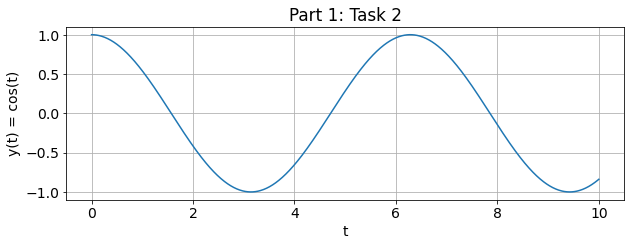
\includegraphics[scale = 0.545]{Part1-Task2.png}\\[1.0 cm]
\end{center}

The step responses achieved with the user-defined convolution function are plotted in the next figure. Considering a general graphical convolution of the first equation with the step function, we would expect the result to grow rapidly at first, then slow before dropping off with the exponential decay. By flipping the second function over the y-axis and shifting it, the hypothesis would be that overlap would accumulate at a steady rate, reach a peak at 6s, and remain at that peak. The third step response should rise and fall in a sinusoidal pattern. \\

While the first and third subplots match these general shapes prescribed, the second shows an obvious deviation. The reason for this difference will be returned to and elaborated on after analyzing the hand-calculated response results. The time interval has been correctly set to cover the time from -20s to 20s. \\

\begin{center}
	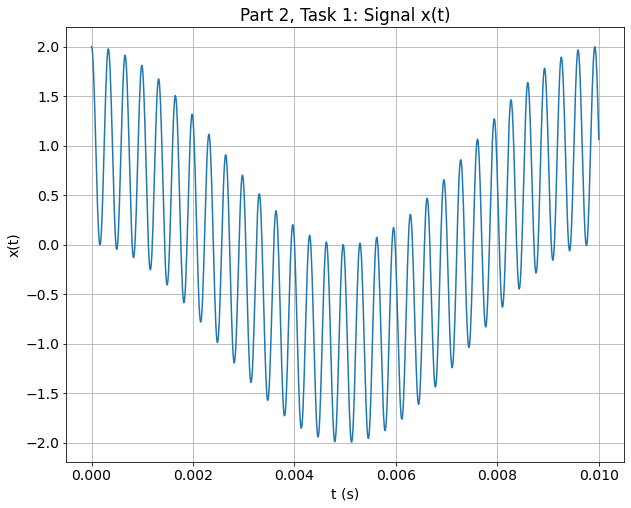
\includegraphics[scale = 0.53]{Part2-Task1.png}\\[1.0 cm]
\end{center}

The solutions to each hand calculation of the step responses for Equations 1-3 are shown below. Considering the general shapes expected from each response discussed in the prior section, these equations would seem to be accurate models. The first is a combination of exponential growth followed by shifted exponential decay. The second shows a steady increase followed by a decrease after a short time. The last convolution provides the suggested sinusoidal shape. The hand result of $ h_2(t) * u(t) $ would support the assertion that the step response plotted with the user-defined convolution function is not fully accurate.

\begin{equation*}
	h_1(t) * u(t) = -0.5(e^{-2t} - 1)u(t) + 0.5(e^{-2(t - 3)} - 1)u(t - 3)
\end{equation*} \\
\begin{equation*}
	h_2(t) * u(t) =	(t - 2)u(t - 2) - (t - 6)u(t - 6)
\end{equation*} \\
\begin{equation*}
	h_3(t) * u(t) =	\frac{1}{w_0} sin(w_0t)u(t)
\end{equation*} \\

The plots created from the hand-derived step response equations are shown in the following figure. Each of the three subplots differs from its counterpart in the plot of Part 2, Task 1. The subplot for $ h_1(t) * u(t) $ shows how the response was stretched along the x-axis over a greater time interval in Task 1. The step response pictured in the middle subplot remains at its peak value here as opposed to falling back to zero. Finally, all three subplots were also stretched along the y-axis previously. \\

Given that these plots in Task 2 are based on mathematical derivations, we can reason that the problem may lie with the Python convolution method. Analyzing the process, it seems that the horizontal and vertical stretching of the functions is caused by the doubling of the array size in order combine the inputs. The fact that Equation 3 contains the regular, unshifted step function explicitly may be why it was spared from the horizontal scaling. \\

An explanation for the difference in the step response of Equation 2 is that the step function itself was bound by the time interval for the convolution. In the hand-calculated equation, the step function did not have this limitation and thus never caused a decrease back to zero. Consequently, the disparity between the results in Part 2 is necessitated by how the convolution was found in Python. With this understanding informing our expectations, the results and their variations make sense. \\

\begin{center}
	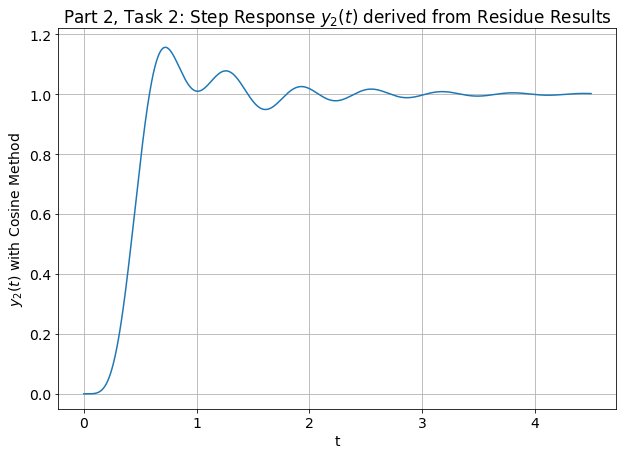
\includegraphics[scale = 0.55]{Part2-Task2.png}\\[1.0 cm]
\end{center}
	
\section{Error Analysis}
	
The primary difficulty I had during this lab was in setting the secondary time interval for the convolution function. I initially tried to double the size by keeping the original lower bound and shifting only to the right. This gave an interval of $ [-10,30] $ rather than the proper time interval of $ [-20,20] $. Since these values were able to produce a plot of the proper shapes, I did not realize the error until I had plotted the hand-calculated equations. The issue caused each result to be shifted right by 10s. I solved this problem by replacing the values -10 and 30 within my np.arange time assignment with -20 and 20.  \\
	
\section{Questions}
	
1. The lab tasks, expectations, and deliverables were largely all communicated clearly in this lab. The time interval for the step response was incorrect, however, specifying an interval of $ [-10,10] $, rather than $ [-20,20] $. \\
	
\section{Conclusion}
	
This lab enabled a greater understanding of the step response and the properties of the convolution implementation in Python. It honed our skills in solving convolutions by hand through further practice, and verified the results of these computations. It challenged our understanding of numpy arrays and the effect of altering their dimensions. \\ 

Despite the different results obtained in Tasks 1 and 2 of Part 2, the plot differences were a remnant of the Python convolution method. In that it challenged our initial expectations and required reasoning to understand the validity of our findings, this lab was very successful. If this lab were repeated, however, I think it would be wise to clue the students in that the plots will not be identical so that they can attempt to independently deduce the cause. \\

Through my initial time interval setup error, I grew to realize the importance of writing code that is portable. Rather than reviewing the implementation and recalculating input values each time the code is repurposed, a generalized setting will be both more efficient and less likely to produce another error. In the future, I will focus on identifying opportunities where a more portable solution could be utilized. \\
	
\newpage
\begin{thebibliography}{111}
		
	\bibitem{S}
Sullivan, Dennis M. (2018) {\it  Signals and Systems for Electrical Engineers I}. Nevada: CreateSpace Independent Publishing Platform.
		
\end{thebibliography}
\end{document}

% Lab Report based on template created by Roza Aceska.